\documentclass[onecolumn]{article} % Use article class, one column

% Standard LaTeX Packages
\usepackage[utf8]{inputenc} % Input encoding
\usepackage[T1]{fontenc}    % Font encoding
\usepackage{amsmath}        % Math formulas
\usepackage{amssymb}        % Math symbols
\usepackage{graphicx}       % Include graphics
\usepackage{hyperref}       % Create hyperlinks
\usepackage{lipsum}         % Dummy text (for placeholder citations)
\usepackage{geometry}       % Added for margin control
\usepackage{tikz}           % Added for TikZ diagrams
\usepackage{float}          % Added for [H] float specifier
\usepackage{algorithm}      % Added for algorithm environment
\usepackage{algorithmic}   % Added for algorithmic environment

% TikZ Libraries
\usetikzlibrary{shapes, arrows.meta, positioning, chains, fit, calc}

% Set margins
\geometry{margin=1in}

% Optional: Customize hyperref appearance
\hypersetup{
    colorlinks=true,
    linkcolor=blue,
    filecolor=magenta,
    urlcolor=cyan,
}

% Placeholder for citation command if needed (replace with actual bibliography setup)
% \newcommand{\cite}[1]{[#1]} % Simple placeholder

% --- Document Information ---
\title{Multi-Scale Temporal Graph Attention Network for Spatiotemporal Forecasting}
\author{Your Name / Affiliation} % Replace with actual author info
\date{\today}

\begin{document}

\maketitle
% Optional: Add abstract environment if needed
% \begin{abstract}
% ...
% \end{abstract}
\tableofcontents % Optional: Add a table of contents

% --- Start of Original Content ---
% Note: \chapter is replaced by \section, \section by \subsection, \subsection by \subsubsection

\section{Introduction} % Chapters start sections numbering from 1. Use \section if you prefer continuous numbering.

Spatiotemporal forecasting presents one of the most significant challenges in machine learning research, requiring models that can simultaneously capture complex spatial relationships and temporal dynamics. This problem is particularly crucial in domains such as epidemiology, where disease spread exhibits intricate patterns across both geographical regions and time periods. Traditional approaches often treat spatial and temporal components separately, failing to model their interdependence and leading to suboptimal predictions. Furthermore, many existing methods rely on predefined graph structures that may not accurately reflect the true underlying relationships in the data.

In this section, we introduce the Multi-Scale Temporal Graph Attention Network (MSTGAT), a novel deep learning architecture specifically designed to address these limitations. MSTGAT integrates several innovative components: (1) efficient feature extraction using depthwise separable convolutions, (2) adaptive graph learning through a low-rank attention mechanism, (3) multi-scale temporal modeling via dilated convolutions, and (4) horizon prediction with an adaptive refinement mechanism.

Our contributions can be summarized as follows:
\begin{itemize}
    \item We propose a comprehensive end-to-end architecture that jointly models spatial dependencies and temporal dynamics at multiple scales.
    \item We introduce a low-rank graph attention mechanism that learns and adapts spatial relationships during training without relying on a predefined adjacency matrix.
    \item We develop a multi-scale temporal module that efficiently captures patterns across different time horizons through dilated convolutions with adaptive fusion.
    \item We design an adaptive refinement mechanism that combines model predictions with recent observations, improving forecasting accuracy particularly during regime changes.
    \item We optimize computational efficiency through strategic use of low-rank approximations and separable convolutions, enabling application to large-scale spatiotemporal forecasting problems.
\end{itemize}

The remainder of this paper is organized as follows: Section \ref{sec:problem} formalizes the spatiotemporal forecasting problem. Section \ref{sec:architecture} presents the proposed MSTGAT architecture in detail. Section \ref{sec:theory} provides theoretical analysis of the model's properties. Section \ref{sec:implementation} discusses practical implementation considerations. Section \ref{sec:variants} explores model variants and ablation studies. Finally, Section \ref{sec:limitations} addresses limitations and future research directions.

\section{Problem Formulation} % Changed from \chapter to \section
\label{sec:problem}

Let us consider $N$ geographical regions (e.g., cities, counties, or states) as nodes in a graph. The historical epidemic or resource usage/demand data is represented as $\mathbf{X} = [\mathbf{x}_1, \mathbf{x}_2, \ldots, \mathbf{x}_t]$, where $\mathbf{x}_z \in \mathbb{R}^N$ denotes the observed case counts across all $N$ regions at time step $z$. For each specific region $i$, its temporal sequence is represented as $\mathbf{x}^i = [x_{i,1}, x_{i,2}, \ldots, x_{i,t}]$.

Our objective is to predict future case values $\mathbf{x}_{t+h}$ for a fixed horizon $h$, which may correspond to different forecasting tasks either short-term or long-term prediction. For any prediction task, we utilise a look-back window of length $T$ to capture relevant historical patterns. Specifically, we use the sequence $[\mathbf{x}_{t-T+1}, \mathbf{x}_{t-T+2}, \ldots, \mathbf{x}_t] \in \mathbb{R}^{N \times T}$ to predict $\mathbf{x}_{t+h}$.

The spatial relationships between regions are encoded in a graph structure $\mathcal{G} = (\mathcal{V}, \mathcal{E}, \mathbf{A})$, where $\mathcal{V} = \{v_1, v_2, \ldots, v_N\}$ represents the set of regions, $\mathcal{E}$ denotes the connections between regions, and $\mathbf{A} \in \mathbb{R}^{N \times N}$ is the adjacency matrix. Each element $a_{ij}$ of $\mathbf{A}$ quantifies the relationship strength between regions $v_i$ and $v_j$.

The forecasting task can then be formalised as learning a function $f$ that maps the historical data and graph structure to future predictions:

\begin{equation}
\hat{\mathbf{x}}_{t+h} = f([\mathbf{x}_{t-T+1}, \mathbf{x}_{t-T+2}, \ldots, \mathbf{x}_t]; \mathcal{G})
\end{equation}

where $\hat{\mathbf{x}}_{t+h}$ represents the predicted case counts for all regions at time $t+h$.

For efficient implementation and training, we adopt a batch-oriented tensor formulation. Let $\mathbf{X} \in \mathbb{R}^{B \times T \times N}$ represent the input tensor, where $B$ is the batch size, $T$ is the historical window length, and $N$ is the number of regions. The forecasting task becomes:

\begin{equation}
\hat{\mathbf{Y}} = \mathcal{F}(\mathbf{X}; \Theta)
\end{equation}

where $\hat{\mathbf{Y}} \in \mathbb{R}^{B \times h \times N}$ contains predictions for all regions across the prediction horizon $h$, and $\Theta$ represents the learnable parameters of the model.

This formulation presents several challenges:
\begin{itemize}
    \item \textbf{Dynamic Spatial Relationships}: The strength and nature of relationships between regions may vary over time and across different epidemic stages.
    \item \textbf{Multi-Scale Temporal Patterns}: Epidemiological data often exhibits patterns at different time scales, from daily fluctuations to weekly seasonality and longer-term trends.
    \item \textbf{Heterogeneity}: Regions may have different baseline characteristics, population densities, and response to interventions.
    \item \textbf{Limited Data}: Especially in emerging epidemics, historical data may be limited, requiring models that can generalize from small datasets.
    \item \textbf{Computational Efficiency}: Models must scale to large numbers of regions and long time series.
\end{itemize}

Our proposed MSTGAT architecture specifically addresses these challenges through its novel components and design principles.

Algorithm \ref{alg:msagatnet_training} outlines the overall training procedure employed for optimizing the MSTGAT model parameters. It follows a standard supervised learning paradigm with mini-batch gradient descent, incorporating validation-based early stopping and learning rate scheduling to ensure robust convergence and prevent overfitting.

\begin{algorithm}[h]
    \caption{MSAGATNet Training Algorithm}
    \label{alg:msagatnet_training}
    \begin{algorithmic}[1]
    \REQUIRE 
        Dataset $\{X,Y\}$ (Input sequences $X$, Target sequences $Y$),
        optional initial Adjacency $A_0$, 
        hyperparameters $(\eta,\lambda,p,\gamma,E)$ (learning rate, weight decay, patience, LR factor, epochs)
    \ENSURE 
        Best model parameters $\Theta^*$ based on validation performance
    \STATE Initialize model parameters $\Theta\!\sim\!{\rm init}$
    \STATE Initialize Optimizer $\mathrm{OPT}\!=\!\mathrm{Adam}(\eta,\lambda)$
    \STATE Initialize LR Scheduler $\mathrm{SCH}\!=\!\mathrm{ReduceLROnPlateau}(p,\gamma)$
    \STATE Initialize best validation loss $L_{\rm val}^* \gets \infty$, patience counter $\mathrm{patience} \gets 0$
    \FOR{$e=1,2,\dots,E$} \hfill\COMMENT{Loop over training epochs}
      \STATE $L_{\rm tr}\gets0$ \hfill\COMMENT{Initialize total training loss for the epoch}
      \FOR{each batch $(X_b,Y_b)$ in training set}
        \STATE $(\hat Y_b,L_{\rm att})\gets\mathrm{MSAGATNet}(X_b,A_0;\Theta)$ \hfill\COMMENT{Forward pass: get predictions and attention loss}
        \STATE $L_b\gets\mathrm{MSE}(\hat Y_b,Y_b)+L_{\rm att}$ \hfill\COMMENT{Compute batch loss (MSE + attention regularization)}
        \STATE Perform backpropagation: Compute gradients $\nabla_\Theta L_b$
        \STATE Update parameters using optimizer: $\Theta\gets\mathrm{OPT.step}(\Theta, \nabla_\Theta L_b)$ \hfill\COMMENT{Gradient descent step}
        \STATE $L_{\rm tr}\mathrel{+}=L_b$ \hfill\COMMENT{Accumulate batch loss}
      \ENDFOR
      \STATE $L_{\rm tr}\gets L_{\rm tr}/|\mathrm{train}|$ \hfill\COMMENT{Calculate average training loss for the epoch}
      \STATE $L_{\rm val}\gets\mathrm{Eval}(\mathrm{valid}, \Theta)$ \hfill\COMMENT{Evaluate model on validation set}
      \STATE $\mathrm{SCH}.step(L_{\rm val})$ \hfill\COMMENT{Update learning rate based on validation loss}
      \IF{$L_{\rm val}<L_{\rm val}^*$} \hfill\COMMENT{Check if validation performance improved}
        \STATE $\Theta^*\gets\Theta$ \hfill\COMMENT{Save best parameters}
        \STATE $L_{\rm val}^*\gets L_{\rm val}$ \hfill\COMMENT{Update best validation loss}
        \STATE $\mathrm{patience}\gets0$ \hfill\COMMENT{Reset patience counter}
        \STATE $\mathrm{Eval}(\mathrm{test},\Theta^*)$ \hfill\COMMENT{Optional: Evaluate best model on test set}
      \ELSE
        \STATE $\mathrm{patience}\mathrel{+}=1$ \hfill\COMMENT{Increment patience counter}
      \ENDIF
      \IF{$\mathrm{patience}\ge p$} \hfill\COMMENT{Check for early stopping condition}
        \STATE \textbf{break} \hfill\COMMENT{Stop training if no improvement for $p$ epochs}
      \ENDIF
    \ENDFOR
    \RETURN $\Theta^*$ \hfill\COMMENT{Return the best performing model parameters}
    \end{algorithmic}
\end{algorithm}

Algorithm \ref{alg:msagatnet_math} provides a detailed mathematical breakdown of the forward pass within the MSTGAT model, illustrating the sequence of operations from input processing to final prediction generation as described conceptually in Section \ref{sec:architecture}.

\begin{algorithm}[h]
  \caption{MSAGATNet: Mathematical Formulation of Forward Pass}
  \label{alg:msagatnet_math}
  \begin{algorithmic}[1]
    \REQUIRE 
      Input batch $X\in\mathbb{R}^{B\times T\times N}$,\quad optional initial Adjacency $A_0\in\mathbb{R}^{N\times N}$
    \ENSURE 
      Predicted batch $\hat{Y}\in\mathbb{R}^{B\times h\times N},\;$ Attention Regularization Loss $L_{\rm att}$
      
    \STATE \textbf{// Feature Extraction Module}
    \STATE $\tilde{X}\!=\!{\rm reshape}(X)\in\mathbb{R}^{BN\times1\times T}$ \hfill\COMMENT{Reshape input for 1D convolution over time}
    \STATE $Z_{\rm dep}=\mathrm{DWConv}(\tilde{X})$ \hfill\COMMENT{Apply depthwise convolution along time}
    \STATE $Z=\mathrm{PWConv}(\sigma\,{\rm BN}(Z_{\rm dep}))$ \hfill\COMMENT{Apply pointwise convolution, BN, activation}
    \STATE $H=\sigma\bigl({\rm LN}( (\text{Flatten}(Z)) W_L W_H+b)\bigr)\in\mathbb{R}^{BN\times D}$ \hfill\COMMENT{Flatten, apply low-rank projection, LN, activation}
    \STATE $H \leftarrow {\rm reshape}(H)\in\mathbb{R}^{B\times N\times D}$ \hfill\COMMENT{Reshape features per node}
    \STATE $X_L=X_{:,-1,:}\in\mathbb{R}^{B\times N}$ \hfill\COMMENT{Extract last observation for prediction refinement}
           
    \STATE \textbf{// Spatial Dependency Module (Simplified Single Head)}
    \STATE $[Q,K,V]=\mathrm{split}(H\,W_{qkv}^L\,W_{qkv}^H+b_{qkv})$ \hfill\COMMENT{Project H to Q, K, V using low-rank layers}
    \STATE $\widetilde{Q}=\mathrm{ELU}(Q)+1,\;\widetilde{K}=\mathrm{ELU}(K)+1$ \hfill\COMMENT{Apply positive mapping (e.g., ELU+1) for linear attention}
    \STATE $A_{\rm bias} = UV^T$ \hfill\COMMENT{Compute low-rank learnable graph bias}
    \STATE $A_{\rm scores} = \frac{\widetilde{Q}\widetilde{K}^T}{\sqrt{D}} + A_{\rm bias} + \lambda A_0$ \hfill\COMMENT{Compute attention scores (content + bias + initial adj.)}
    \STATE $A = \mathrm{softmax}(A_{\rm scores})$ \hfill\COMMENT{Compute final attention matrix}
    \STATE $O = A V$ \hfill\COMMENT{Standard attention: Aggregate values based on attention (can be replaced by linear approx.)}
    % \STATE $O=\dfrac{\widetilde{Q}\,( \widetilde{K}^T V )}{\sum_j\widetilde{K}_j+\epsilon}$ \hfill\COMMENT{Optional: Linear attention computation for efficiency}
    \STATE $H_s = \mathrm{LN}( (OW_o^L\,W_o^H + b_o) + H )$ \hfill\COMMENT{Low-rank output projection, add residual, apply LayerNorm}
    \STATE $L_{\rm att}=\lambda_{\rm att}\|A\|_1$ \hfill\COMMENT{Calculate attention regularization loss (e.g., L1 norm)}
    
    \STATE \textbf{// Multi-Scale Temporal Module}
    \STATE Initialize list $Z_{scales} = []$
    \FOR{$s=1,\dots,S$}
      \STATE $Z_s=\mathrm{Drop}\bigl(\sigma\,{\rm BN}(\mathrm{Conv1D}(H_s^T,\,d=2^{s-1}))\bigr)$ \hfill\COMMENT{Apply dilated Conv1D for scale $s$}
      \STATE Append $Z_s$ to $Z_{scales}$
    \ENDFOR
    \STATE $\alpha=\mathrm{softmax}(w)$ \hfill\COMMENT{Compute adaptive fusion weights for scales}
    \STATE $Z = \sum_{s=1}^S \alpha_s Z_{scales}[s]$ \hfill\COMMENT{Weighted sum fusion of scale features}
    \STATE $H_t=\mathrm{LN}( (Z^T W_f^L\,W_f^H + b_f) + H_s )$ \hfill\COMMENT{Low-rank fusion projection, add residual, apply LayerNorm}
    
    \STATE \textbf{// Horizon Prediction Module}
    \STATE $P=\mathrm{Predictor}(H_t)$ \hfill\COMMENT{Generate initial prediction using bottleneck MLP}
    \STATE $G=\mathrm{sigmoid}(\mathrm{GateMLP}(H_t))$ \hfill\COMMENT{Compute adaptive gate values using MLP}
    \STATE $E=X_L\odot\exp(-\beta\,[1:h])$ \hfill\COMMENT{Compute time-decayed extrapolation from last observation}
    \STATE $\hat{Y}_{B,N,h}=G\odot P+(1-G)\odot E$ \hfill\COMMENT{Combine prediction and extrapolation using gate}
    \STATE $\hat{Y} = \text{Transpose}(\hat{Y}_{B,N,h})$ \hfill\COMMENT{Transpose to final shape $\mathbb{R}^{B\times h\times N}$}
  \end{algorithmic}
\end{algorithm}
    

\section{MSTGAT Architecture} % Changed from \chapter to \section
\label{sec:architecture}

\subsection{Architectural Overview} % Changed from \section to \subsection

The Multi-Scale Temporal Graph Attention Network (MSTGAT) is conceived as a modular, end-to-end deep learning architecture specifically tailored for the complexities of spatiotemporal forecasting. Its design focuses on effectively capturing both spatial dependencies between entities (e.g., geographical regions) and temporal dynamics within their time series data, while maintaining computational efficiency. Figure \ref{fig:architecture} provides a high-level schematic of the model's structure and information flow.

\begin{figure}[htbp]
    \centering
    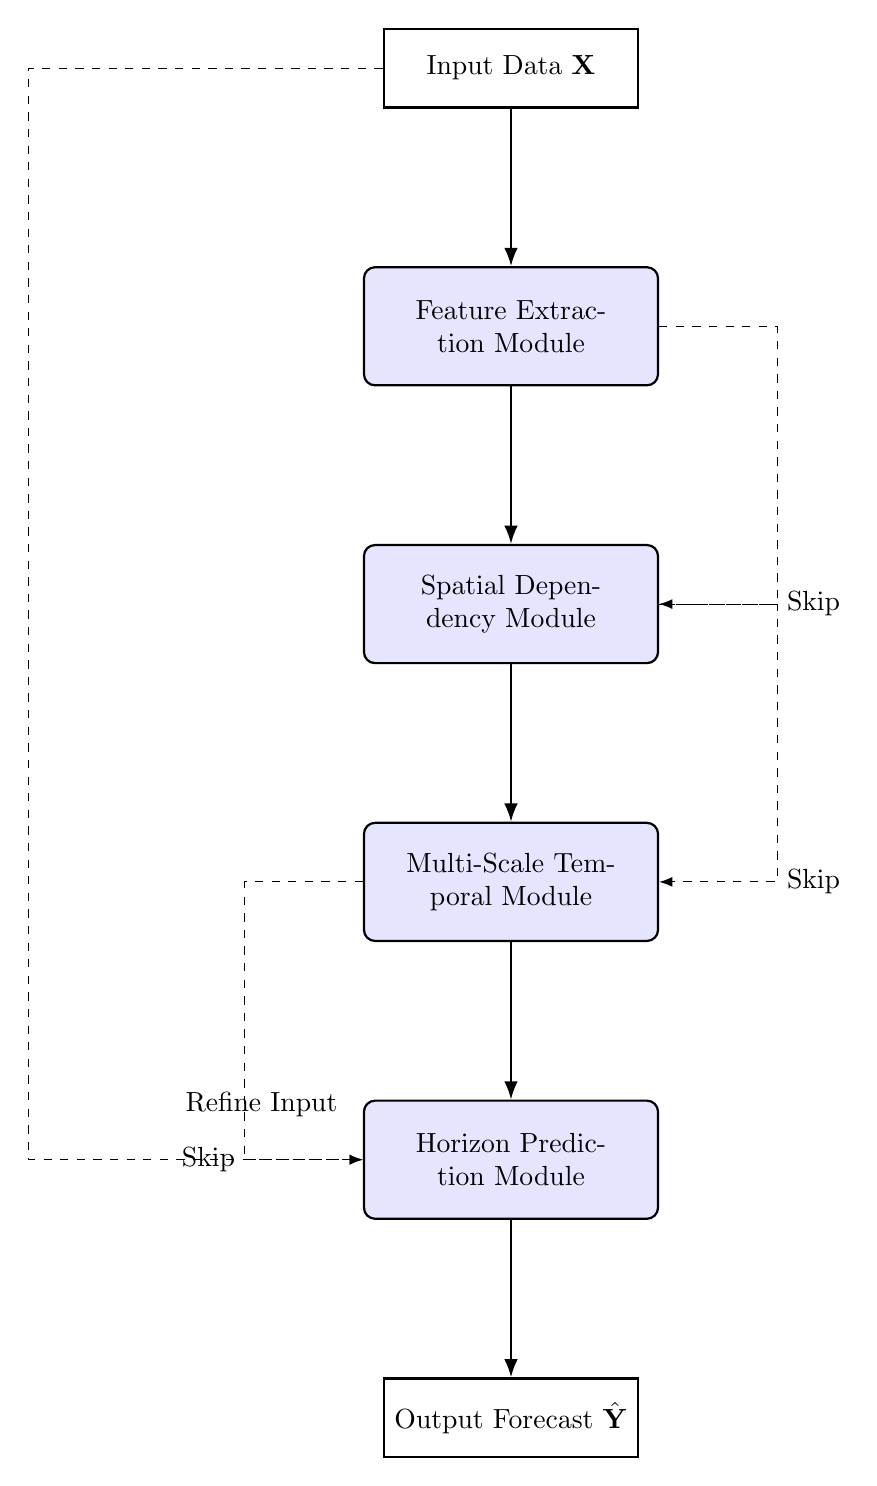
\begin{tikzpicture}[node distance=2cm and 3cm, >=Latex, 
        module/.style={rectangle, draw, thick, text centered, rounded corners, minimum height=1.5cm, text width=3.5cm, fill=blue!10},
        input/.style={rectangle, draw, thick, text centered, minimum height=1cm, text width=3cm},
        output/.style={rectangle, draw, thick, text centered, minimum height=1cm, text width=3cm},
        point/.style={coordinate}]
    
        \node (input) [input] {Input Data $\mathbf{X}$}; 
        \node (feat_ext) [module, below=of input] {Feature Extraction Module};
        \node (spatial) [module, below=of feat_ext] {Spatial Dependency Module};
        \node (temporal) [module, below=of spatial] {Multi-Scale Temporal Module};
        \node (predict) [module, below=of temporal] {Horizon Prediction Module};
        \node (output) [output, below=of predict] {Output Forecast $\hat{\mathbf{Y}}$};
        
        % Main flow
        \draw [->, thick] (input) -- (feat_ext);
        \draw [->, thick] (feat_ext) -- (spatial);
        \draw [->, thick] (spatial) -- (temporal);
        \draw [->, thick] (temporal) -- (predict);
        \draw [->, thick] (predict) -- (output);
        
        % Skip connections (dotted)
        \node (skip1_start) [point, right=1.5cm of feat_ext] {};
        \node (skip1_end) [point, right=1.5cm of spatial] {};
        \draw [->, dashed] (feat_ext.east) -| (skip1_end) |- (spatial.east) node[pos=0.25, right] {Skip};
    
        \node (skip2_start) [point, right=1.5cm of spatial] {};
        \node (skip2_end) [point, right=1.5cm of temporal] {};
        \draw [->, dashed] (spatial.east) -| (skip2_end) |- (temporal.east) node[pos=0.25, right] {Skip};
    
        \node (skip3_start) [point, left=1.5cm of temporal] {};
        \node (skip3_end) [point, left=1.5cm of predict] {};
        \draw [->, dashed] (temporal.west) -| (skip3_end) |- (predict.west) node[pos=-0.5, left] {Skip};
    
        % Input to Prediction Module (for refinement)
        \node (input_refine) [point, left=4cm of predict] {};
        \draw [->, dashed] (input.west) -- ++(-4.5,0) |- (input_refine) -- (predict.west) node[pos=0.95, above=20pt, left] {Refine Input};
    
    \end{tikzpicture}
    \caption{Overall architecture of the proposed MSTGAT model. The framework consists of four key components: Feature Extraction Module, Spatial Dependency Module, Multi-Scale Temporal Module, and Horizon Prediction Module. Dashed lines indicate skip connections and input for refinement.}
    \label{fig:architecture}
\end{figure}

At its core, MSTGAT processes the input tensor $\mathbf{X} \in \mathbb{R}^{B \times T \times N}$ (Batch Size $\times$ Time Steps $\times$ Nodes) through four primary, sequential modules, each designed to address a specific aspect of the spatiotemporal forecasting problem:

\begin{enumerate}
    \item \textbf{Feature Extraction}: Transforms raw time series into latent representations that capture relevant patterns.
    \item \textbf{Spatial Dependency Modeling}: Captures relationships between different regions through an adaptive graph attention mechanism.
    \item \textbf{Multi-Scale Temporal Modeling}: Models temporal dynamics at different time scales through dilated convolutions.
    \item \textbf{Horizon Prediction}: Generates forecasts for future time steps with an adaptive refinement mechanism.
\end{enumerate}

The architecture is underpinned by several key design principles aimed at enhancing performance and practicality:
\begin{itemize}
    \item \textbf{Parameter Efficiency}: We employ low-rank decompositions and separable convolutions to reduce the number of parameters and computational complexity.
    \item \textbf{Adaptive Learning}: Rather than relying on fixed graph structures or pre-specified temporal dependencies, the model learns and adapts these relationships during training.
    \item \textbf{Multi-Scale Processing}: We explicitly model patterns at different temporal scales to capture both short-term fluctuations and long-term trends.
    \item \textbf{Residual Learning}: Skip connections throughout the architecture facilitate gradient flow and information propagation.
\end{itemize}

We now delve into the specifics of each module, detailing its function, underlying mechanisms, and contribution to the overall model.

\subsection{Feature Extraction Module} % Changed from \section to \subsection
\label{sec:feature_extraction}

The primary role of the feature extraction module is to transform the raw input time series data for each node into a more informative and compact latent representation. This initial stage is crucial for preparing the data for the subsequent, more complex spatial and temporal modeling steps. It aims to:

\begin{itemize}
    \item Extract meaningful features from potentially noisy time series data
    \item Maintain locality of temporal patterns
    \item Process large volumes of data efficiently
    \item Create representations that are suitable for subsequent spatial and temporal modeling
\end{itemize}

\subsubsection{Input Transformation} % Changed from \subsection to \subsubsection

Given the input tensor $\mathbf{X} \in \mathbb{R}^{B \times T \times N}$, we first reshape it to facilitate convolution operations:

\begin{equation}
\mathbf{X}' = \text{Reshape}(\mathbf{X}) \in \mathbb{R}^{BN \times 1 \times T}
\end{equation}

This transformation allows us to process each region's time series independently in the initial stage. The dimension $1$ corresponds to the input channel dimension for the convolution operation.

\subsubsection{Depthwise Separable Convolutions} % Changed from \subsection to \subsubsection

Traditional convolutional neural networks (CNNs) apply full convolutions that operate across both the spatial (in our case, region) and channel dimensions simultaneously. This approach becomes computationally expensive as the number of regions and channels increases. Instead, we employ depthwise separable convolutions, which factorize the standard convolution operation into two more efficient steps:

\begin{enumerate}
    \item \textbf{Depthwise Convolution}: This operation applies a separate filter to each input channel, thereby capturing temporal patterns within each channel independently:

    \begin{equation}
    \mathbf{Z}_{dep}(i, j, k) = \sum_{m=1}^{K} \mathbf{X}'(i, j, k+m-\lfloor \frac{K+1}{2} \rfloor) \cdot \mathbf{W}_{dep}(j, 1, m)
    \end{equation}

    where $\mathbf{W}_{dep} \in \mathbb{R}^{1 \times 1 \times K}$ is the depthwise convolutional kernel with kernel size $K$, $i$ indexes the batch dimension, $j$ indexes the channel dimension, and $k$ indexes the temporal dimension.

    \item \textbf{Pointwise Convolution}: This is a $1 \times 1$ convolution that projects the output of the depthwise convolution across channels:

    \begin{equation}
    \mathbf{Z}_{pw}(i, c_{out}, k) = \sum_{c_{in}=1}^{C_{in}} \mathbf{Z}_{dep}(i, c_{in}, k) \cdot \mathbf{W}_{pw}(c_{out}, c_{in}, 1)
    \end{equation}

    where $\mathbf{W}_{pw} \in \mathbb{R}^{C_{out} \times C_{in} \times 1}$ is the pointwise convolutional kernel, $C_{in}$ is the number of input channels (1 in our case), and $C_{out}$ is the number of output channels.
\end{enumerate}

The complete depthwise separable convolution operation can be expressed as:

\begin{equation}
\mathbf{Z} = \text{DSConv}(\mathbf{X}') = \text{PWConv}(\text{DWConv}(\mathbf{X}'))
\end{equation}

We enhance this operation with batch normalization and nonlinear activation:

\begin{equation}
\mathbf{Z}_{bn} = \text{BN}(\mathbf{Z})
\end{equation}

\begin{equation}
\mathbf{Z}_{act} = \sigma(\mathbf{Z}_{bn})
\end{equation}

where $\sigma$ represents the ReLU activation function and BN denotes batch normalization.

This approach offers several advantages:
\begin{itemize}
    \item \textbf{Computational Efficiency}: Reduces the number of operations from $\mathcal{O}(C_{in} \cdot C_{out} \cdot K \cdot T)$ for standard convolution to $\mathcal{O}(C_{in} \cdot K \cdot T + C_{in} \cdot C_{out})$ for depthwise separable convolution.
    \item \textbf{Parameter Efficiency}: Reduces the number of parameters from $C_{in} \cdot C_{out} \cdot K$ to $C_{in} \cdot K + C_{in} \cdot C_{out}$.
    \item \textbf{Regularization Effect}: The factorization provides an implicit regularization effect, potentially improving generalization.
\end{itemize}

The resulting tensor $\mathbf{Z}_{act} \in \mathbb{R}^{BN \times C_{out} \times T}$ contains rich temporal features extracted from the input data.

\subsubsection{Low-Rank Feature Projection} % Changed from \subsection to \subsubsection

To further enhance computational efficiency and reduce the risk of overfitting, we employ a low-rank bottleneck projection. This approach is particularly valuable in spatiotemporal forecasting, where data may be limited and high-dimensional representations can lead to overfitting.

The extracted features $\mathbf{Z}_{act}$ are first flattened along the temporal dimension:

\begin{equation}
\mathbf{Z}_{flat} = \text{Flatten}(\mathbf{Z}_{act}) \in \mathbb{R}^{BN \times (C_{out} \cdot T)}
\end{equation}

We then project these features through a bottleneck architecture:

\begin{equation}
\mathbf{H}_{low} = \mathbf{Z}_{flat}\mathbf{W}_{low} + \mathbf{b}_{low} \in \mathbb{R}^{BN \times D_{low}}
\end{equation}

\begin{equation}
\mathbf{H}_{high} = \mathbf{H}_{low}\mathbf{W}_{high} + \mathbf{b}_{high} \in \mathbb{R}^{BN \times D}
\end{equation}

\begin{equation}
\mathbf{H} = \sigma(\text{LN}(\mathbf{H}_{high})) \in \mathbb{R}^{BN \times D}
\end{equation}

where $D_{low}$ represents the bottleneck dimensionality, $D$ is the hidden dimensionality, $\mathbf{W}_{low} \in \mathbb{R}^{(C_{out} \cdot T) \times D_{low}}$ and $\mathbf{W}_{high} \in \mathbb{R}^{D_{low} \cdot D}$ are the projection matrices, $\mathbf{b}_{low} \in \mathbb{R}^{D_{low}}$ and $\mathbf{b}_{high} \in \mathbb{R}^{D}$ are bias terms, LN denotes layer normalization, and $\sigma$ is the ReLU activation function.

Finally, we reshape $\mathbf{H}$ back to a form suitable for spatial modeling:

\begin{equation}
\mathbf{H}_{reshaped} = \text{Reshape}(\mathbf{H}) \in \mathbb{R}^{B \times N \times D}
\end{equation}

This bottleneck architecture serves multiple purposes:
\begin{itemize}
    \item \textbf{Dimensionality Reduction}: Reduces the feature dimensionality from $C_{out} \cdot T$ to $D$, where typically $D < C_{out} \cdot T$, decreasing the number of parameters in subsequent layers.
    \item \textbf{Information Distillation}: Forces the model to extract essential features by compressing information through the bottleneck.
    \item \textbf{Improved Gradient Flow}: The low-rank projection can help mitigate vanishing gradient problems.
    \item \textbf{Enhanced Generalization}: The reduced parameter space helps prevent overfitting, particularly valuable in epidemiological forecasting where data may be limited.
\end{itemize}

The computational complexity of this projection is $\mathcal{O}(BN \cdot C_{out} \cdot T \cdot D_{low} + BN \cdot D_{low} \cdot D)$, compared to $\mathcal{O}(BN \cdot C_{out} \cdot T \cdot D)$ for a direct projection, representing significant savings when $D_{low} \ll \min(C_{out} \cdot T, D)$.

\subsubsection{Theoretical Insights on Feature Extraction} % Changed from \subsection to \subsubsection

The feature extraction module can be understood from several theoretical perspectives:

\textbf{Signal Processing Perspective}: The depthwise convolution acts as a set of learned filters that extract temporal patterns at different frequencies. By applying separate filters to each input channel, the model can capture channel-specific patterns. The pointwise convolution then integrates information across channels, similar to a learned cross-channel correlation.

\textbf{Information Bottleneck Perspective}: The low-rank projection can be viewed through the lens of the information bottleneck principle \cite{tishby2000information}. By compressing the representation to a lower-dimensional space, the model is forced to retain only the most predictive features, discarding irrelevant information. This leads to representations that are both minimal and sufficient for the forecasting task.

\textbf{Manifold Learning Perspective}: Epidemiological data often lies on a low-dimensional manifold within the high-dimensional observation space. The bottleneck projection can be seen as learning this manifold, with $D_{low}$ representing its intrinsic dimensionality.

\subsection{Spatial Dependency Modeling} % Changed from \section to \subsection
\label{sec:spatial_modeling}

Following feature extraction, the spatial dependency module focuses on capturing and modeling the relationships *between* different nodes (regions) at a given time step. A critical aspect of MSTGAT is its ability to learn these spatial relationships adaptively from the data, rather than relying solely on predefined, static graph structures (like geographical adjacency). This adaptivity is vital in domains like epidemiology where interactions can be complex and dynamic.

\begin{figure}[htbp]
\centering
% Replace includegraphics with improved TikZ diagram
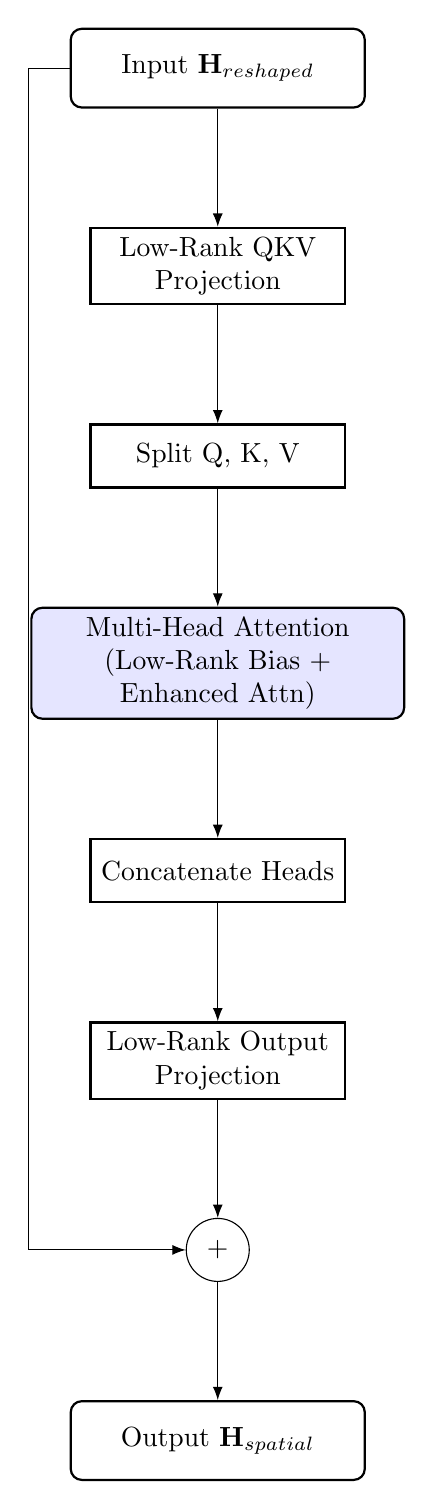
\begin{tikzpicture}[node distance=1.5cm and 2cm, >=Latex, 
    block/.style={rectangle, draw, thick, text centered, rounded corners, minimum height=1cm, text width=3.5cm},
    op/.style={rectangle, draw, thick, text centered, minimum height=0.8cm, text width=3cm},
    attn/.style={rectangle, draw, thick, text centered, rounded corners, minimum height=1cm, text width=4.5cm, fill=blue!10},
    point/.style={coordinate},
    sum/.style={circle, draw, minimum size=0.8cm}]

    \node (input) [block] {Input $\mathbf{H}_{reshaped}$}; 
    \node (lr_qkv) [op, below=of input] {Low-Rank QKV Projection};
    \node (split) [op, below=of lr_qkv] {Split Q, K, V};
    \node (mha) [attn, below=of split] {Multi-Head Attention\\(Low-Rank Bias + Enhanced Attn)};
    \node (concat) [op, below=of mha] {Concatenate Heads};
    \node (lr_out) [op, below=of concat] {Low-Rank Output Projection};
    \node (sum) [sum, below=of lr_out] {+};
    \node (output) [block, below=of sum] {Output $\mathbf{H}_{spatial}$};
    \node (res_start) [point, left=2cm of sum] {};

    \draw [->] (input) -- (lr_qkv);
    \draw [->] (lr_qkv) -- (split);
    \draw [->] (split) -- (mha);
    \draw [->] (mha) -- (concat);
    \draw [->] (concat) -- (lr_out);
    \draw [->] (lr_out) -- (sum);
    \draw [->] (sum) -- (output);
    \draw [->] (input.west) -| (res_start) |- (sum);

\end{tikzpicture}
\caption{Diagram of the Spatial Dependency Modeling Module (TikZ). The module learns adaptive spatial relationships through multi-head attention with a low-rank bias term.}
\label{fig:spatial_module}
\end{figure}

After feature extraction, we model spatial dependencies using a novel graph attention mechanism. Unlike conventional graph neural networks that rely on a predefined adjacency matrix, our approach learns and adapts the spatial relationships during training. This is particularly valuable in epidemiological forecasting, where the true underlying spatial relationships may be unknown or may evolve over time.

\subsubsection{Motivation and Theoretical Foundations} % Changed from \subsection to \subsubsection

Traditional graph-based models for spatiotemporal forecasting typically rely on fixed graph structures derived from geographical proximity, transportation networks, or other domain knowledge. However, these predefined structures may not accurately capture the complex dependencies in epidemic spread, which can be influenced by factors such as:

\begin{itemize}
    \item Population mobility patterns
    \item Socioeconomic factors
    \item Healthcare resource distribution
    \item Intervention policies
    \item Environmental conditions
\end{itemize}

Furthermore, these dependencies may evolve over the course of an epidemic. Our approach draws inspiration from graph attention networks (GAT) \cite{velivckovic2017graph} and transformer architectures \cite{vaswani2017attention}, but introduces several innovations to address the specific challenges of spatiotemporal forecasting.

\subsubsection{Low-Rank Graph Attention} % Changed from \subsection to \subsubsection

The core of our spatial modeling is a multi-head attention mechanism with low-rank decomposition. For clarity, we first describe the process for a single attention head and then extend it to the multi-head case.

Given the node features $\mathbf{H}_{reshaped} \in \mathbb{R}^{B \times N \times D}$ from the feature extraction module, we first project them to obtain query, key, and value representations. To maintain computational efficiency, we use a low-rank projection:

\begin{equation}
\mathbf{QKV}_{low} = \mathbf{H}_{reshaped}\mathbf{W}_{qkv\_low} + \mathbf{b}_{qkv\_low} \in \mathbb{R}^{B \times N \times 3D_{low}}
\end{equation}

\begin{equation}
\mathbf{QKV} = \mathbf{QKV}_{low}\mathbf{W}_{qkv\_high} + \mathbf{b}_{qkv\_high} \in \mathbb{R}^{B \times N \times 3D}
\end{equation}

where $\mathbf{W}_{qkv\_low} \in \mathbb{R}^{D \times 3D_{low}}$, $\mathbf{W}_{qkv\_high} \in \mathbb{R}^{3D_{low} \times 3D}$, and $\mathbf{b}_{qkv\_low} \in \mathbb{R}^{3D_{low}}$, $\mathbf{b}_{qkv\_high} \in \mathbb{R}^{3D}$ are learnable parameters.

We then split $\mathbf{QKV}$ into query, key, and value representations:

\begin{equation}
\mathbf{Q}, \mathbf{K}, \mathbf{V} = \text{Split}(\mathbf{QKV}) \in \mathbb{R}^{B \times N \times D} \times \mathbb{R}^{B \times N \times D} \times \mathbb{R}^{B \times N \times D}
\end{equation}

For multi-head attention with $H$ heads, we reshape these tensors:

\begin{equation}
\mathbf{Q}_h, \mathbf{K}_h, \mathbf{V}_h = \text{Reshape}(\mathbf{Q}, \mathbf{K}, \mathbf{V}) \in \mathbb{R}^{B \times H \times N \times \frac{D}{H}} \times \mathbb{R}^{B \times H \times N \times \frac{D}{H}} \times \mathbb{R}^{B \times H \times N \times \frac{D}{H}}
\end{equation}

\subsubsection{Learnable Graph Structure} % Changed from \subsection to \subsubsection

A key innovation in our approach is the incorporation of a learnable graph structure, complementing the content-based attention. Rather than computing attention scores based solely on the query-key interactions, we introduce a learnable bias term that encodes underlying graph structural information. This bias is parameterized efficiently using a low-rank factorization:

\begin{equation}
\mathbf{U}_h \in \mathbb{R}^{N \times D_{low}}, \mathbf{V}_h \in \mathbb{R}^{D_{low} \times N}
\end{equation}

\begin{equation}
\mathbf{A}_{bias,h} = \mathbf{U}_h\mathbf{V}_h \in \mathbb{R}^{N \times N}
\end{equation}

where $\mathbf{U}_h$ and $\mathbf{V}_h$ are learnable embedding matrices for each attention head $h$. This low-rank formulation is crucial for parameter efficiency, reducing the number of parameters required to represent the graph structure from $\mathcal{O}(N^2)$ (for a full matrix) to $\mathcal{O}(N \cdot D_{low})$. This makes it feasible to learn meaningful graph structures even for large numbers of nodes, capturing potentially complex, non-local relationships that might be missed by predefined graphs.

The attention scores are then computed as:

\begin{equation}
\mathbf{A}_{raw,h} = \frac{\mathbf{Q}_h\mathbf{K}_h^T}{\sqrt{D/H}} + \mathbf{A}_{bias,h} \in \mathbb{R}^{B \times H \times N \times N}
\end{equation}

\begin{equation}
\mathbf{A}_h = \text{softmax}(\mathbf{A}_{raw,h}) \in \mathbb{R}^{B \times H \times N \times N}
\end{equation}

where the softmax is applied along the last dimension. The scaling factor $\sqrt{D/H}$ helps stabilize training by preventing the attention scores from becoming too concentrated.

\subsubsection{Enhanced Attention Mechanism} % Changed from \subsection to \subsubsection

To further enhance the attention mechanism, we incorporate a nonlinear transformation inspired by the ELU (Exponential Linear Unit) activation function. This helps capture more complex relationships between nodes:

\begin{equation}
\tilde{\mathbf{Q}}_h = \text{ELU}(\mathbf{Q}_h) + 1.0
\end{equation}

\begin{equation}
\tilde{\mathbf{K}}_h = \text{ELU}(\mathbf{K}_h) + 1.0
\end{equation}

The addition of 1.0 ensures that the transformed values are positive, which is important for the stability of the attention mechanism. We then compute key-value products:

\begin{equation}
\mathbf{KV}_h = \tilde{\mathbf{K}}_h \otimes \mathbf{V}_h \in \mathbb{R}^{B \times H \times \frac{D}{H} \times \frac{D}{H}}
\end{equation}

where $\otimes$ represents the batched outer product operation.

To ensure proper normalization, we compute a normalization factor:

\begin{equation}
\mathbf{z}_h = \frac{1}{\sum_{j=1}^{N} \tilde{\mathbf{K}}_h(j) + \epsilon} \in \mathbb{R}^{B \times H \times N}
\end{equation}

where $\epsilon$ is a small constant for numerical stability. The attended features are then computed as:

\begin{equation}
\mathbf{O}_h = \tilde{\mathbf{Q}}_h \otimes \mathbf{KV}_h \otimes \mathbf{z}_h \in \mathbb{R}^{B \times H \times N \times \frac{D}{H}}
\end{equation}

\subsubsection{Output Projection and Residual Connection} % Changed from \subsection to \subsubsection

The outputs from all heads are concatenated and projected back to the original dimension:

\begin{equation}
\mathbf{O} = \text{Concat}(\mathbf{O}_1, \mathbf{O}_2, \ldots, \mathbf{O}_H) \in \mathbb{R}^{B \times N \times D}
\end{equation}

To maintain computational efficiency, we again use a low-rank projection:

\begin{equation}
\mathbf{O}_{low} = \mathbf{O}\mathbf{W}_{out\_low} + \mathbf{b}_{out\_low} \in \mathbb{R}^{B \times N \times D_{low}}
\end{equation}

\begin{equation}
\mathbf{O}_{high} = \mathbf{O}_{low}\mathbf{W}_{out\_high} + \mathbf{b}_{out\_high} \in \mathbb{R}^{B \times N \times D}
\end{equation}

Finally, we apply a residual connection to facilitate gradient flow:

\begin{equation}
\mathbf{H}_{spatial} = \mathbf{O}_{high} + \mathbf{H}_{reshaped} \in \mathbb{R}^{B \times N \times D}
\end{equation}

\subsubsection{Attention Regularization} % Changed from \subsection to \subsubsection

To encourage sparsity in the learned attention weights and prevent overfitting to spurious spatial correlations, we apply L1 regularization to the attention matrix:

\begin{equation}
\mathcal{L}_{attn} = \lambda_{attn} \sum_{h=1}^{H} \|\mathbf{A}_h\|_1
\end{equation}

where $\lambda_{attn}$ is a hyperparameter controlling the regularization strength. This regularization term is added to the overall loss function during training.

\subsubsection{Interpretability of Learned Spatial Relationships} % Changed from \subsection to \subsubsection

A significant advantage of our approach is the interpretability of the learned attention weights. The attention matrix $\mathbf{A}_h$ provides insights into the spatial relationships learned by the model. Specifically, $\mathbf{A}_h(i,j)$ represents the influence of region $j$ on region $i$ in the prediction process.

By visualizing these attention weights, we can:
\begin{itemize}
    \item Identify key transmission pathways in epidemic spread
    \item Discover unexpected spatial relationships that might not be captured by geographical proximity
    \item Monitor how spatial dependencies evolve over the course of an epidemic
    \item Validate the model's learned relationships against domain knowledge
\end{itemize}

This interpretability is particularly valuable in epidemiological applications, where understanding the spatial patterns of disease spread is crucial for intervention planning.

\subsection{Multi-Scale Temporal Modeling} % Changed from \section to \subsection
\label{sec:temporal_modeling}

Once spatial dependencies have been incorporated into the node representations, the multi-scale temporal module processes the sequence of representations along the time dimension. Its primary goal is to capture temporal patterns and dependencies occurring at various time scales, ranging from short-term fluctuations to longer-term trends. This is achieved efficiently through the use of dilated convolutions.

\begin{figure}[h!]
\centering
% Improved multi-scale diagram with spacing and scale
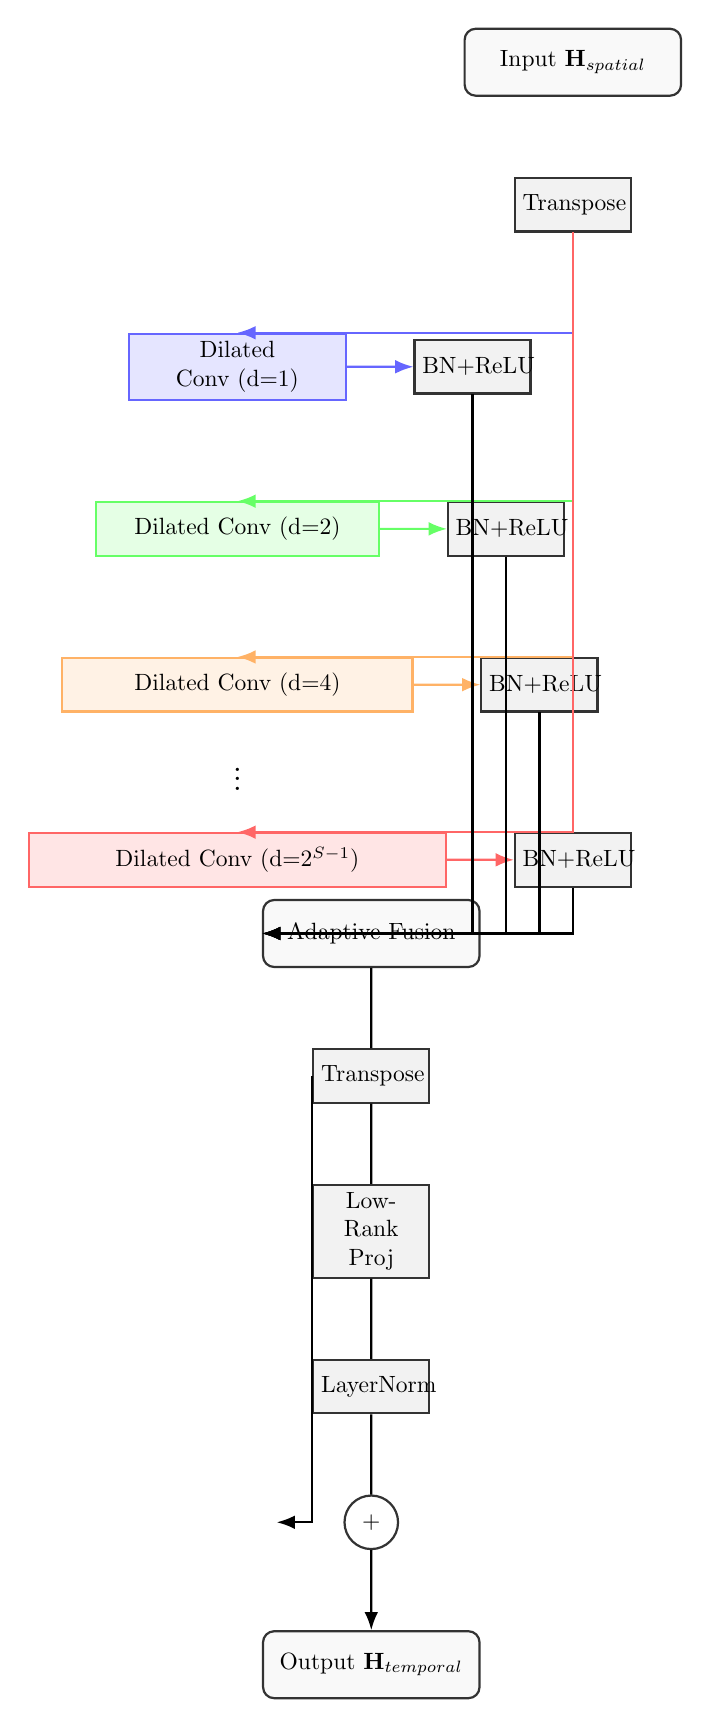
\begin{tikzpicture}[scale=0.85, transform shape, node distance=1.2cm and 1.8cm, >=Latex,
    scale1/.style={rectangle, draw=blue!60, thick, text centered, minimum height=0.8cm, text width=3cm, fill=blue!10},
    scale2/.style={rectangle, draw=green!60, thick, text centered, minimum height=0.8cm, text width=4cm, fill=green!10},
    scale3/.style={rectangle, draw=orange!60, thick, text centered, minimum height=0.8cm, text width=5cm, fill=orange!10},
    scaleS/.style={rectangle, draw=red!60, thick, text centered, minimum height=0.8cm, text width=6cm, fill=red!10},
    proc/.style={rectangle, draw=black!80, thick, text centered, minimum height=0.8cm, text width=1.5cm, fill=gray!10},
    block/.style={rectangle, draw=black!80, thick, text centered, rounded corners, minimum height=1cm, text width=3cm, fill=gray!5}]

    \node (input) [block] {Input $\mathbf{H}_{spatial}$};
    \node (trans) [proc, below=of input] {Transpose};
    
    \node (s1) [scale1, below left=1.5cm and 2.5cm of trans] {Dilated Conv (d=1)};
    \node (b1) [proc, right=1cm of s1] {BN+ReLU};
    \draw[->, blue!60, thick] (s1) -- (b1);
    \draw[->, blue!60, thick] (trans.south) |- (s1.north);
    
    \node (s2) [scale2, below=1.5cm of s1] {Dilated Conv (d=2)};
    \node (b2) [proc, right=1cm of s2] {BN+ReLU};
    \draw[->, green!60, thick] (s2) -- (b2);
    \draw[->, green!60, thick] (trans.south) |- (s2.north);
    
    \node (s3) [scale3, below=1.5cm of s2] {Dilated Conv (d=4)};
    \node (b3) [proc, right=1cm of s3] {BN+ReLU};
    \draw[->, orange!60, thick] (s3) -- (b3);
    \draw[->, orange!60, thick] (trans.south) |- (s3.north);
    
    \node (dots) [below=0.5cm of s3] {\Large $\vdots$};
    
    \node (sS) [scaleS, below=0.5cm of dots] {Dilated Conv (d=$2^{S-1}$)};
    \node (bS) [proc, right=1cm of sS] {BN+ReLU};
    \draw[->, red!60, thick] (sS) -- (bS);
    \draw[->, red!60, thick] (trans.south) |- (sS.north);
    
    \node (fus) [block, below=1.5cm of dots, xshift=2cm] {Adaptive Fusion};
    %% merge
    \draw[->, thick] (b1.south) |- (fus.west);
    \draw[->, thick] (b2.south) |- (fus.west);
    \draw[->, thick] (b3.south) |- (fus.west);
    \draw[->, thick] (bS.south) |- (fus.west);
    
    \node (trans2) [proc, below=of fus] {Transpose};
    \node (lrp) [proc, below=of trans2] {Low-Rank Proj};
    \node (ln) [proc, below=of lrp] {LayerNorm};
    \node (sum2) [circle, draw=black!80, thick, minimum size=0.8cm, below=of ln] {+};
    \node (out) [block, below=of sum2] {Output $\mathbf{H}_{temporal}$};
    \draw[->, thick] (fus) -- (trans2) -- (lrp) -- (ln) -- (sum2) -- (out);
    \draw[->, thick] (trans2.west) |- ([xshift=-1cm]sum2.west);

\end{tikzpicture}
\caption{Multi-Scale Temporal Module (scaled). Colored paths indicate different dilation scales for clarity.}
\label{fig:temporal_module}
\end{figure}

The temporal dynamics of epidemiological data often exhibit patterns at different time scales, from daily fluctuations to weekly seasonality and longer-term trends. Traditional approaches that focus on a single time scale may fail to capture the full spectrum of temporal dependencies. Our multi-scale temporal module addresses this challenge through dilated convolutions and adaptive fusion.

\subsubsection{Motivation and Theoretical Foundations} % Changed from \subsection to \subsubsection

Epidemiological time series exhibit complex temporal patterns influenced by various factors:
\begin{itemize}
    \item \textbf{Short-term fluctuations}: Day-to-day variations due to testing patterns, reporting delays, and random noise
    \item \textbf{Medium-term patterns}: Weekly seasonality, incubation periods, and intermediate-term effects of interventions
    \item \textbf{Long-term trends}: Overall epidemic trajectory, seasonal effects, and long-term policy impacts
\end{itemize}

Capturing these multi-scale patterns requires a model that can efficiently process information at different temporal resolutions. Dilated convolutions \cite{yu2015multi} provide an elegant solution to this challenge, offering an exponentially increasing receptive field with linear parameter growth.

\subsubsection{Multi-Scale Dilated Convolutions} % Changed from \subsection to \subsubsection

The core of our temporal modeling is a set of dilated convolutions with increasing dilation rates. Given the spatial features $\mathbf{H}_{spatial} \in \mathbb{R}^{B \times N \times D}$, we first reshape them to facilitate temporal convolution operations:

\begin{equation}
\mathbf{H}_{temp} = \text{Transpose}(\mathbf{H}_{spatial}) \in \mathbb{R}^{B \times D \times N}
\end{equation}

For each scale $s \in \{1, 2, \ldots, S\}$, we apply a dilated convolution with dilation rate $2^{s-1}$:

\begin{equation}
\mathbf{Z}_s = \text{Conv1D}(\mathbf{H}_{temp}, \text{kernel\_size}=K, \text{dilation}=2^{s-1}, \text{padding}=(K-1) \cdot 2^{s-1} / 2) \in \mathbb{R}^{B \times D \times N}
\end{equation}

\begin{equation}
\mathbf{Z}_{s,bn} = \text{BatchNorm1D}(\mathbf{Z}_s) \in \mathbb{R}^{B \times D \times N}
\end{equation}

\begin{equation}
\mathbf{Z}_{s,act} = \sigma(\mathbf{Z}_{s,bn}) \in \mathbb{R}^{B \times D \times N}
\end{equation}

\begin{equation}
\mathbf{Z}_{s,drop} = \text{Dropout}(\mathbf{Z}_{s,act}, p=p_{drop}) \in \mathbb{R}^{B \times D \times N}
\end{equation}

where $K$ is the kernel size, $\sigma$ is the ReLU activation function, and $p_{drop}$ is the dropout probability.

The dilation rates create an exponentially increasing receptive field:
\begin{itemize}
    \item Scale 1 (dilation = 1): Receptive field of size $K$
    \item Scale 2 (dilation = 2): Receptive field of size $K + (K-1)$
    \item Scale 3 (dilation = 4): Receptive field of size $K + 3(K-1)$
    \item Scale s (dilation = $2^{s-1}$): Receptive field of size $K + (2^s - 1)(K-1)$
\end{itemize}

This allows the model to efficiently capture dependencies at different time scales without the need for deep architectures, addressing the vanishing gradient problem often encountered in modeling long-term dependencies.

\subsubsection{Adaptive Fusion Mechanism} % Changed from \subsection to \subsubsection

Different temporal scales may have varying importance depending on the specific forecasting task, epidemic stage, or region characteristics. Rather than using fixed weights to combine the multi-scale features, we employ an adaptive fusion mechanism with learnable parameters:

\begin{equation}
\mathbf{w} \in \mathbb{R}^S
\end{equation}

\begin{equation}
\boldsymbol{\alpha} = \text{softmax}(\mathbf{w}) \in \mathbb{R}^S
\end{equation}

The features from different scales are then combined using these weights:

\begin{equation}
\mathbf{Z}_{fused} = \sum_{s=1}^{S} \alpha_s \mathbf{Z}_{s,drop} \in \mathbb{R}^{B \times D \times N}
\end{equation}

This adaptive fusion allows the model to focus on the most relevant temporal scales for each forecasting task. For example, short-term forecasting may rely more on recent patterns, while long-term forecasting may give more weight to broader trends.

\subsubsection{Low-Rank Projection and Residual Connection} % Changed from \subsection to \subsubsection

Similar to previous modules, we apply a low-rank projection to maintain computational efficiency:

\begin{equation}
\mathbf{Z}_{fused}^T = \text{Transpose}(\mathbf{Z}_{fused}) \in \mathbb{R}^{B \times N \times D}
\end{equation}

\begin{equation}
\mathbf{Z}_{low} = \mathbf{Z}_{fused}^T\mathbf{W}_{fusion\_low} + \mathbf{b}_{fusion\_low} \in \mathbb{R}^{B \times N \times D_{low}}
\end{equation}

\begin{equation}
\mathbf{Z}_{high} = \mathbf{Z}_{low}\mathbf{W}_{fusion\_high} + \mathbf{b}_{fusion\_high} \in \mathbb{R}^{B \times N \times D}
\end{equation}

We then apply layer normalization and a residual connection:

\begin{equation}
\mathbf{H}_{temporal} = \text{LayerNorm}(\mathbf{Z}_{high} + \mathbf{Z}_{fused}^T) \in \mathbb{R}^{B \times N \times D}
\end{equation}

The residual connection helps maintain gradient flow during training, while the layer normalization stabilizes the training process.

\subsubsection{Theoretical Insights on Multi-Scale Temporal Modeling} % Changed from \subsection to \subsubsection

The multi-scale temporal module can be understood from several theoretical perspectives:

\textbf{Wavelet Transform Perspective}: The dilated convolutions can be viewed as analogous to a learnable wavelet transform, which decomposes the signal into components at different scales. The adaptive fusion then reconstructs the signal by combining these components with learned weights.

\begin{equation}
\mathbf{H}_{temporal} = \text{LayerNorm}(\mathbf{Z}_{high} + \mathbf{Z}_{fused}^T) \in \mathbb{R}^{B \times N \times D}
\end{equation}

The residual connection helps maintain gradient flow during training, while the layer normalization stabilizes the training process.

\subsubsection{Theoretical Insights on Multi-Scale Temporal Modeling} % Changed from \subsection to \subsubsection

The multi-scale temporal module can be understood from several theoretical perspectives:

\textbf{Wavelet Transform Perspective}: The dilated convolutions can be viewed as analogous to a learnable wavelet transform, which decomposes the signal into components at different scales. The adaptive fusion then reconstructs the signal by combining these components with learned weights.

\textbf{Hierarchical Processing Perspective}: The different scales create a hierarchical representation of the temporal dynamics, with lower scales capturing local patterns and higher scales capturing global trends. This hierarchical structure is well-suited to the multi-scale nature of epidemiological data.

\textbf{Memory Capacity Perspective}: The exponentially increasing receptive field allows the model to efficiently memorize patterns at different time scales, similar to how long short-term memory (LSTM) networks maintain multiple time scales of memory but with a more computationally efficient architecture.

\subsection{Horizon Prediction with Adaptive Refinement} % Changed from \section to \subsection
\label{sec:prediction}

% Add figure for Horizon Prediction Module
\begin{figure}[htbp]
\centering
% Improved Horizon Prediction Module diagram with better spacing and scale
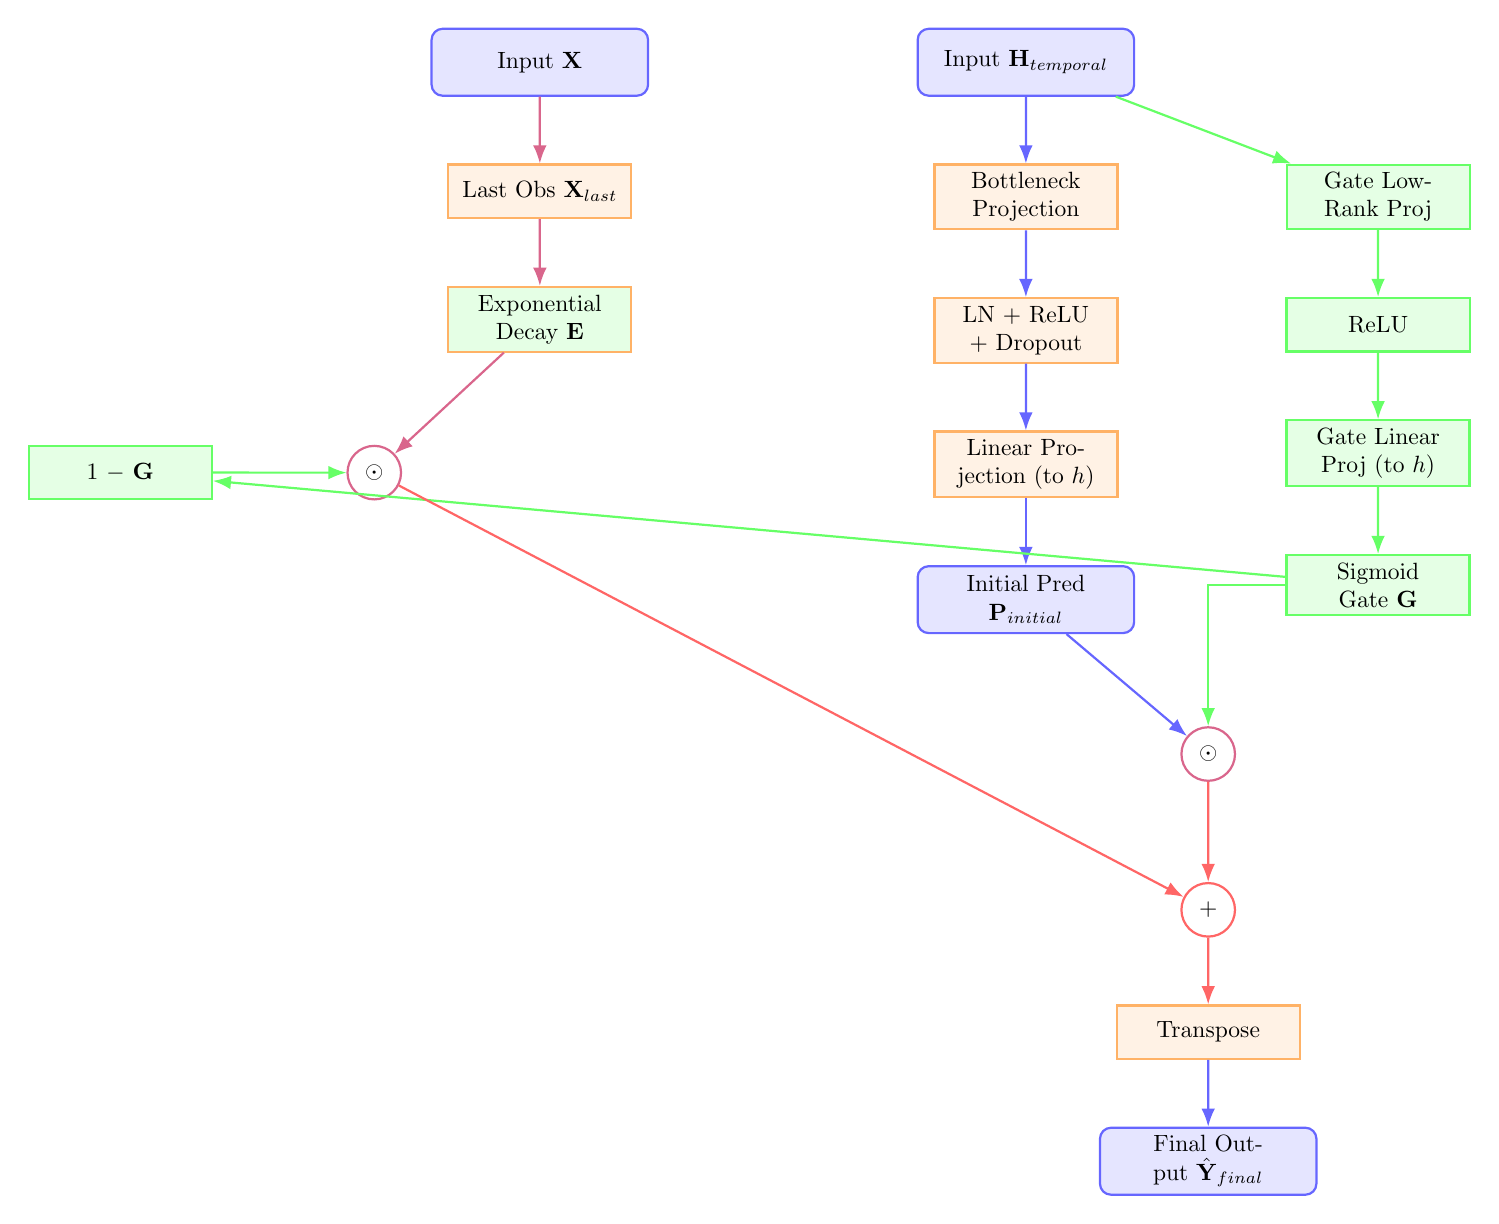
\begin{tikzpicture}[scale=0.85, transform shape, node distance=1cm and 1.8cm, >=Latex,
    block/.style={rectangle, draw=blue!60, thick, text centered, rounded corners, minimum height=1cm, text width=3cm, fill=blue!10},
    op/.style={rectangle, draw=orange!60, thick, text centered, minimum height=0.8cm, text width=2.5cm, fill=orange!10},
    gate/.style={rectangle, draw=green!60, thick, text centered, minimum height=0.8cm, text width=2.5cm, fill=green!10},
    prod/.style={circle, draw=purple!60, thick, minimum size=0.8cm, inner sep=0pt, label=center:$\odot$},
    sum/.style={circle, draw=red!60, thick, minimum size=0.8cm}]

    \node (input_h) [block] {Input $\mathbf{H}_{temporal}$};
    \node (input_x) [block, left=4cm of input_h] {Input $\mathbf{X}$};
    
    % Prediction Path
    \node (pred_lr1) [op, below=of input_h] {Bottleneck Projection};
    \node (pred_ln) [op, below=of pred_lr1] {LN + ReLU + Dropout};
    \node (pred_lr2) [op, below=of pred_ln] {Linear Projection (to $h$)};
    \node (p_initial) [block, below=of pred_lr2, fill=blue!10] {Initial Pred $\mathbf{P}_{initial}$};

    % Gate Path
    \node (gate_lr1) [gate, right=2.5cm of pred_lr1] {Gate Low-Rank Proj};
    \node (gate_act) [gate, below=of gate_lr1] {ReLU};
    \node (gate_lr2) [gate, below=of gate_act] {Gate Linear Proj (to $h$)};
    \node (gate_sig) [gate, below=of gate_lr2] {Sigmoid Gate $\mathbf{G}$};

    % Decay Path
    \node (last_obs) [op, below=of input_x] {Last Obs $\mathbf{X}_{last}$};
    \node (exp_decay) [op, below=of last_obs, fill=green!10] {Exponential Decay $\mathbf{E}$};
    
    % Fusion
    \node (prod_p) [prod, below right=1.5cm and 0.8cm of p_initial] {};
    \node (prod_e) [prod, below left=1.5cm and 0.8cm of exp_decay] {};
    \node (gate_inv) [gate, left=2cm of prod_e] {$1-\mathbf{G}$};
    \node (sum) [sum, below=1.5cm of prod_p] {+};
    \node (transpose) [op, below=of sum] {Transpose};
    \node (output) [block, below=of transpose] {Final Output $\hat{\mathbf{Y}}_{final}$};

    % Connections
    \draw[->, blue!60, thick] (input_h) -- (pred_lr1);
    \draw[->, blue!60, thick] (pred_lr1) -- (pred_ln);
    \draw[->, blue!60, thick] (pred_ln) -- (pred_lr2);
    \draw[->, blue!60, thick] (pred_lr2) -- (p_initial);
    
    \draw[->, green!60, thick] (input_h) -- (gate_lr1);
    \draw[->, green!60, thick] (gate_lr1) -- (gate_act);
    \draw[->, green!60, thick] (gate_act) -- (gate_lr2);
    \draw[->, green!60, thick] (gate_lr2) -- (gate_sig);
    
    \draw[->, purple!60, thick] (input_x) -- (last_obs);
    \draw[->, purple!60, thick] (last_obs) -- (exp_decay);
    
    \draw[->, blue!60, thick] (p_initial) -- (prod_p);
    \draw[->, green!60, thick] (gate_sig) -| (prod_p);
    
    \draw[->, purple!60, thick] (exp_decay) -- (prod_e);
    \draw[->, green!60, thick] (gate_sig) -- (gate_inv);
    \draw[->, green!60, thick] (gate_inv) -- (prod_e);
    
    \draw[->, red!60, thick] (prod_p) -- (sum);
    \draw[->, red!60, thick] (prod_e) -- (sum);
    \draw[->, red!60, thick] (sum) -- (transpose);
    \draw[->, blue!60, thick] (transpose) -- (output);

\end{tikzpicture}
\caption{Diagram of the Horizon Prediction Module (scaled). The module combines predictions and decay via colored pathways for clarity.}
\label{fig:prediction_module}
\end{figure}

The final component of our MSTGAT architecture is the horizon prediction module, which generates forecasts for future time steps. This module combines the rich spatiotemporal representations from previous layers with an adaptive refinement mechanism that leverages the most recent observations.

\subsubsection{Motivation} % Changed from \subsection to \subsubsection

Epidemiological forecasting faces several challenges:
\begin{itemize}
    \item \textbf{Regime Changes}: Sudden shifts in epidemic dynamics due to policy changes, variant emergence, or behavioral adaptations
    \item \textbf{Uncertainty Growth}: Prediction uncertainty typically increases with the forecast horizon
    \item \textbf{Baseline Drift}: The baseline level may shift over time due to changes in testing, reporting, or population immunity
\end{itemize}

These challenges motivate our adaptive refinement approach, which combines model predictions with an extrapolation from the most recent observations. This hybrid approach allows the model to adapt more quickly to regime changes while maintaining its ability to capture complex spatiotemporal patterns.

\subsubsection{Bottleneck Prediction Architecture} % Changed from \subsection to \subsubsection

Given the temporal features $\mathbf{H}_{temporal} \in \mathbb{R}^{B \times N \times D}$, we first apply a bottleneck architecture to generate initial predictions:

\begin{equation}
\mathbf{P}_{low} = \mathbf{H}_{temporal}\mathbf{W}_{pred\_low} + \mathbf{b}_{pred\_low} \in \mathbb{R}^{B \times N \times D_{low}}
\end{equation}

\begin{equation}
\mathbf{P}_{mid} = \text{LayerNorm}(\mathbf{P}_{low}) \in \mathbb{R}^{B \times N \times D_{low}}
\end{equation}

\begin{equation}
\mathbf{P}_{mid\_act} = \sigma(\mathbf{P}_{mid}) \in \mathbb{R}^{B \times N \times D_{low}}
\end{equation}

\begin{equation}
\mathbf{P}_{mid\_drop} = \text{Dropout}(\mathbf{P}_{mid\_act}, p=p_{drop}) \in \mathbb{R}^{B \times N \times D_{low}}
\end{equation}

\begin{equation}
\mathbf{P}_{initial} = \mathbf{P}_{mid\_drop}\mathbf{W}_{pred\_high} + \mathbf{b}_{pred\_high} \in \mathbb{R}^{B \times N \times h}
\end{equation}

where $h$ is the prediction horizon, $\mathbf{W}_{pred\_low} \in \mathbb{R}^{D \times D_{low}}$, $\mathbf{W}_{pred\_high} \in \mathbb{R}^{D_{low} \times h}$, $\mathbf{b}_{pred\_low} \in \mathbb{R}^{D_{low}}$, and $\mathbf{b}_{pred\_high} \in \mathbb{R}^{h}$ are learnable parameters, and $p_{drop}$ is the dropout probability.

\subsubsection{Adaptive Refinement Gate} % Changed from \subsection to \subsubsection

The key innovation in our prediction module is the adaptive refinement mechanism, which combines the model's initial predictions with an extrapolation from the most recent observations. This is particularly valuable in epidemiological forecasting, where the most recent data points often provide crucial information about current trends.

First, we extract the last observed values from the input data:

\begin{equation}
\mathbf{X}_{last} = \mathbf{X}[:, -1, :] \in \mathbb{R}^{B \times N}
\end{equation}

We then compute a gating mechanism that determines the relative importance of the model predictions versus the recent trend:

\begin{equation}
\mathbf{G}_{low} = \mathbf{H}_{temporal}\mathbf{W}_{gate\_low} + \mathbf{b}_{gate\_low} \in \mathbb{R}^{B \times N \times D_{low}}
\end{equation}

\begin{equation}
\mathbf{G}_{act} = \sigma(\mathbf{G}_{low}) \in \mathbb{R}^{B \times N \times D_{low}}
\end{equation}

\begin{equation}
\mathbf{G} = \text{sigmoid}(\mathbf{G}_{act}\mathbf{W}_{gate\_high} + \mathbf{b}_{gate\_high}) \in \mathbb{R}^{B \times N \times h}
\end{equation}

where $\mathbf{W}_{gate\_low} \in \mathbb{R}^{D \times D_{low}}$, $\mathbf{W}_{gate\_high} \in \mathbb{R}^{D_{low} \times h}$, $\mathbf{b}_{gate\_low} \in \mathbb{R}^{D_{low}}$, and $\mathbf{b}_{gate\_high} \in \mathbb{R}^{h}$ are learnable parameters, and $\sigma$ is the ReLU activation function.

\subsubsection{Exponential Decay from Last Observation} % Changed from \subsection to \subsubsection

We model the extrapolation from the most recent observations using an exponential decay function. This simple yet effective approach captures the natural tendency of many processes to revert to a baseline level over time:

\begin{equation}
\mathbf{T} = [1, 2, \ldots, h] \in \mathbb{R}^h
\end{equation}

\begin{equation}
\mathbf{X}_{last\_expanded} = \mathbf{X}_{last}.unsqueeze(-1) \in \mathbb{R}^{B \times N \times 1}
\end{equation}

\begin{equation}
\mathbf{E} = \mathbf{X}_{last\_expanded} \cdot \exp(-\beta \cdot \mathbf{T}) \in \mathbb{R}^{B \times N \times h}
\end{equation}

where $\beta$ is a decay factor (typically set to 0.1). This exponential decay function provides a simple but effective baseline that assumes the epidemic will gradually stabilize from its current level.

\subsubsection{Adaptive Fusion of Predictions} % Changed from \subsection to \subsubsection

The final predictions are obtained by adaptively combining the model's initial predictions with the exponential decay based on the computed gate values:

\begin{equation}
\hat{\mathbf{Y}} = \mathbf{G} \odot \mathbf{P}_{initial} + (1 - \mathbf{G}) \odot \mathbf{E} \in \mathbb{R}^{B \times N \times h}
\end{equation}

where $\odot$ denotes element-wise multiplication.

We typically transpose the result to match the expected output format:

\begin{equation}
\hat{\mathbf{Y}}_{final} = \text{Transpose}(\hat{\mathbf{Y}}, \text{dim1}=1, \text{dim2}=2) \in \mathbb{R}^{B \times h \times N}
\end{equation}

\subsubsection{Theoretical Insights on Adaptive Refinement} % Changed from \subsection to \subsubsection

The adaptive refinement mechanism can be understood from several perspectives:

\textbf{Ensemble Learning Perspective}: The mechanism effectively creates a dynamic ensemble of two forecasting approaches: a complex spatiotemporal model and a simple exponential decay. The gating mechanism learns to weight these approaches based on the specific context, potentially achieving better performance than either approach alone.

\textbf{Regime Change Adaptation}: During stable periods, the model may rely more on its learned patterns (high gate values). During regime changes or unusual events, it may give more weight to the recent trend (low gate values), allowing faster adaptation to new conditions.

\textbf{Uncertainty Calibration}: The mechanism implicitly incorporates uncertainty in the forecasting process. When the model is uncertain about its predictions (e.g., for longer horizons or unusual patterns), it may rely more on the simple exponential decay, providing a form of regularization.

\subsection{Integration of Components and Information Flow} % Changed from \section to \subsection

The power of MSTGAT lies in the complementary interaction between its spatial and temporal components. While traditional approaches often model these dependencies separately, our architecture allows them to mutually reinforce each other:

\begin{itemize}
    \item The feature extraction module captures local temporal patterns at each node independently, creating a foundation for subsequent spatial and temporal modeling.

    \item The spatial attention module then contextualizes these features by aggregating information across connected nodes, enhancing each node's representation with relevant neighborhood information. This process captures how the epidemic in one region affects and is affected by other regions.

    \item The temporal module subsequently processes these spatially-enriched features across multiple time scales, allowing the model to capture how spatial patterns evolve over time. This acknowledges that spatial dependencies themselves may change at different temporal scales and stages of an epidemic.

    \item Finally, the prediction module combines all this information to generate forecasts, with an adaptive refinement mechanism that balances the complex spatiotemporal patterns learned by the model with a simple extrapolation from recent observations.
\end{itemize}

This bidirectional information flow between spatial and temporal domains is crucial for phenomena like epidemics, where spatial proximity affects transmission timing, and temporal patterns (like mobility) affect spatial spread.

\section{Theoretical Analysis} % Changed from \chapter to \section
\label{sec:theory}

In this section, we present a theoretical analysis of MSTGAT, focusing on its expressivity, computational complexity, and memory requirements.

\subsection{Expressivity Analysis} % Changed from \section to \subsection

The expressivity of a model refers to its ability to represent complex functions or patterns. MSTGAT's expressivity can be analyzed along several dimensions:

\subsubsection{Spatial Expressivity} % Changed from \subsection to \subsubsection

The graph attention mechanism in MSTGAT can represent arbitrary pairwise relationships between regions. The combination of content-based attention (derived from query-key interactions) and learnable graph structure (through the low-rank bias term) allows the model to capture both static geographical relationships and dynamic interaction patterns.

Specifically, for any true underlying adjacency matrix $\mathbf{A}^* \in \mathbb{R}^{N \times N}$, there exists a setting of the parameters $\mathbf{U}_h$ and $\mathbf{V}_h$ such that $\mathbf{U}_h\mathbf{V}_h$ approximates $\mathbf{A}^*$ with a reconstruction error bounded by:

\begin{equation}
\|\mathbf{A}^* - \mathbf{U}_h\mathbf{V}_h\|_F \leq \sqrt{\sum_{i=D_{low}+1}^{N} \sigma_i^2(\mathbf{A}^*)}
\end{equation}

where $\sigma_i(\mathbf{A}^*)$ is the $i$-th singular value of $\mathbf{A}^*$. This error decreases as $D_{low}$ increases, providing a clear trade-off between approximation accuracy and computational efficiency.

\subsubsection{Temporal Expressivity} % Changed from \subsection to \subsubsection

The multi-scale temporal module captures patterns at different time scales through dilated convolutions. The exponentially increasing receptive field allows the model to efficiently represent both short-term and long-term dependencies.

For a temporal sequence of length $T$, the maximum receptive field size with $S$ scales and kernel size $K$ is:

\begin{equation}
R_{\max} = K + (2^S - 1)(K-1)
\end{equation}

This allows the model to capture dependencies spanning a large portion of the input sequence with a relatively small number of scales. For example, with $K=3$ and $S=4$, the model can capture dependencies spanning 27 time steps.

\subsubsection{Combined Spatiotemporal Expressivity} % Changed from \subsection to \subsubsection

The sequential processing of spatial and temporal dependencies in MSTGAT enables it to capture complex spatiotemporal patterns. The composition of these modules allows the model to represent functions that depend on both the spatial configuration and temporal evolution of the data.

More formally, MSTGAT can approximate functions of the form:

\begin{equation}
f(\mathbf{X}) = g(\phi_S(\phi_T(\mathbf{X})))
\end{equation}

where $\phi_T$ captures temporal patterns, $\phi_S$ captures spatial relationships, and $g$ is the prediction function. This compositional structure allows the model to capture how spatial patterns evolve over time and how temporal patterns vary across space.

\subsection{Computational Complexity Analysis} % Changed from \section to \subsection

The computational efficiency of MSTGAT is a key consideration for its applicability to large-scale spatiotemporal forecasting problems. We analyze the computational complexity of each component and the overall model:

\subsubsection{Feature Extraction Module} % Changed from \subsection to \subsubsection

The depthwise separable convolution reduces the computational complexity compared to standard convolution:

\begin{equation}
\mathcal{O}(BN \cdot 1 \cdot K \cdot T + BN \cdot 1 \cdot C_{out}) = \mathcal{O}(BN \cdot (K \cdot T + C_{out}))
\end{equation}

The low-rank projection has a complexity of:

\begin{equation}
\mathcal{O}(BN \cdot C_{out} \cdot T \cdot D_{low} + BN \cdot D_{low} \cdot D)
\end{equation}

\subsubsection{Spatial Attention Module} % Changed from \subsection to \subsubsection

The computation of query, key, and value representations has a complexity of:

\begin{equation}
\mathcal{O}(BN \cdot D \cdot 3D_{low} + BN \cdot 3D_{low} \cdot 3D) = \mathcal{O}(BN \cdot D \cdot D_{low} + BN \cdot D_{low} \cdot D)
\end{equation}

The attention computation has a complexity of:

\begin{equation}
\mathcal{O}(BH \cdot N^2 \cdot D/H) = \mathcal{O}(BN^2 \cdot D)
\end{equation}

The low-rank graph structure adds a complexity of:

\begin{equation}
\mathcal{O}(H \cdot N \cdot D_{low} + H \cdot D_{low} \cdot N) = \mathcal{O}(H \cdot N \cdot D_{low})
\end{equation}

\subsubsection{Temporal Module} % Changed from \subsection to \subsubsection

Each dilated convolution has a complexity of:

\begin{equation}
\mathcal{O}(BN \cdot D \cdot K) = \mathcal{O}(BN \cdot D \cdot K)
\end{equation}

With $S$ scales, the total complexity is:

\begin{equation}
\mathcal{O}(S \cdot BN \cdot D \cdot K)
\end{equation}

The adaptive fusion has a complexity of:

\begin{equation}
\mathcal{O}(BN \cdot D \cdot S)
\end{equation}

\subsubsection{Prediction Module} % Changed from \subsection to \subsubsection

The bottleneck prediction has a complexity of:

\begin{equation}
\mathcal{O}(BN \cdot D \cdot D_{low} + BN \cdot D_{low} \cdot h)
\end{equation}

The adaptive refinement has a complexity of:

\begin{equation}
\mathcal{O}(BN \cdot D \cdot D_{low} + BN \cdot D_{low} \cdot h + BN \cdot h)
\end{equation}

\subsubsection{Overall Complexity} % Changed from \subsection to \subsubsection

The overall computational complexity of MSTGAT is dominated by the attention computation in the spatial module:

\begin{equation}
\mathcal{O}(BN^2 \cdot D)
\end{equation}

This quadratic dependence on the number of nodes $N$ is a common characteristic of attention-based models. However, our low-rank formulations throughout the architecture significantly reduce the constant factors in this complexity, making the model practical for moderate-sized problems.

For very large numbers of nodes, further optimizations such as sparse attention or hierarchical approaches could be considered, but these are beyond the scope of the current work.

\subsection{Memory Requirements Analysis} % Changed from \section to \subsection

The memory requirements of MSTGAT are an important consideration for its practical implementation. We analyze the memory requirements for parameters and activations:

\subsubsection{Parameter Memory} % Changed from \subsection to \subsubsection

The total number of parameters in MSTGAT can be summarized as:

\begin{itemize}
    \item Feature Extraction: $\mathcal{O}(K + C_{out} + C_{out} \cdot T \cdot D_{low} + D_{low} \cdot D)$
    \item Spatial Attention: $\mathcal{O}(D \cdot D_{low} + D_{low} \cdot D + H \cdot N \cdot D_{low})$
    \item Temporal Module: $\mathcal{O}(S \cdot D \cdot K + S + D \cdot D_{low} + D_{low} \cdot D)$
    \item Prediction Module: $\mathcal{O}(D \cdot D_{low} + D_{low} \cdot h + D \cdot D_{low} + D_{low} \cdot h)$
\end{itemize}

The total parameter count is dominated by the $\mathcal{O}(H \cdot N \cdot D_{low})$ term from the low-rank graph structure. However, this is significantly less than the $\mathcal{O}(N^2)$ parameters required for a full adjacency matrix.

\subsubsection{Activation Memory} % Changed from \subsection to \subsubsection

The peak activation memory during forward and backward passes is determined by the largest intermediate tensors, which occur in the attention computation:

\begin{equation}
\mathcal{O}(BH \cdot N^2)
\end{equation}

This quadratic dependence on the number of nodes can be a limiting factor for very large graphs. Techniques such as gradient checkpointing or attention approximation could be used to reduce this memory requirement if needed.

\section{Implementation Considerations} % Changed from \chapter to \section
\label{sec:implementation}

The successful application of MSTGAT to real-world spatiotemporal forecasting problems requires careful consideration of several implementation aspects:

\subsection{Data Preprocessing} % Changed from \section to \subsection

Epidemiological data often requires significant preprocessing due to issues such as:
\begin{itemize}
    \item Missing values
    \item Reporting delays and artifacts
    \item Different scales across regions
    \item Outliers and data quality issues
\end{itemize}

We recommend the following preprocessing steps:
\begin{itemize}
    \item \textbf{Handling Missing Values}: Use interpolation for isolated missing values and more sophisticated techniques such as matrix completion for structured missingness.
    \item \textbf{Normalization}: Scale the data to similar ranges across regions, either through z-score normalization or relative to population size.
    \item \textbf{Smoothing}: Apply moving average or other smoothing techniques to reduce noise, especially for smaller regions with higher variance.
    \item \textbf{Lag Alignment}: Adjust for reporting delays by aligning data based on report dates rather than event dates when necessary.
\end{itemize}

\subsection{Training Strategies} % Changed from \section to \subsection

Training MSTGAT effectively requires careful attention to several aspects:

\subsubsection{Loss Function} % Changed from \subsection to \subsubsection

While mean squared error (MSE) is commonly used for time series forecasting, epidemiological forecasting may benefit from specialized loss functions:

\begin{equation}
\mathcal{L}_{combined} = \alpha \cdot \mathcal{L}_{MSE} + (1-\alpha) \cdot \mathcal{L}_{MAPE} + \gamma \cdot \mathcal{L}_{attn}
\end{equation}

where $\mathcal{L}_{MSE}$ is the mean squared error, $\mathcal{L}_{MAPE}$ is the mean absolute percentage error, $\mathcal{L}_{attn}$ is the attention regularization term, and $\alpha$ and $\gamma$ are hyperparameters.

This combined loss addresses both absolute errors (important for larger regions) and relative errors (important for smaller regions).

\subsubsection{Learning Rate Schedule} % Changed from \subsection to \subsubsection

We recommend a learning rate schedule with initial warmup followed by cosine decay:

\begin{equation}
\eta(t) =
\begin{cases}
\eta_{base} \cdot \frac{t}{T_{warmup}} & \text{if } t < T_{warmup} \\
\eta_{base} \cdot \frac{1 + \cos(\pi \cdot \frac{t - T_{warmup}}{T_{total} - T_{warmup}})}{2} & \text{otherwise}
\end{cases}
\end{equation}

where $\eta_{base}$ is the base learning rate, $T_{warmup}$ is the warmup period, and $T_{total}$ is the total number of training steps.

\subsubsection{Gradient Clipping} % Changed from \subsection to \subsubsection

To stabilize training, especially in the early stages, we recommend gradient clipping:

\begin{equation}
\|\nabla\| = \min(\|\nabla\|, C_{clip})
\end{equation}

where $C_{clip}$ is the gradient clipping threshold.

\subsubsection{Training Regime} % Changed from \subsection to \subsubsection

For epidemiological forecasting, we recommend a sliding window approach:
\begin{itemize}
    \item Split the data into training, validation, and test sets chronologically
    \item Use a sliding window approach to generate multiple training samples from each time series
    \item Ensure no data leakage by maintaining strict temporal separation between training, validation, and test sets
    \item Consider using region-based cross-validation to assess generalization to unseen regions
\end{itemize}

\subsection{Hyperparameter Selection} % Changed from \section to \subsection

Key hyperparameters for MSTGAT include:
\begin{itemize}
    \item \textbf{Architecture Parameters}: Hidden dimension $D$, bottleneck dimension $D_{low}$, number of attention heads $H$, number of temporal scales $S$, kernel size $K$
    \item \textbf{Regularization Parameters}: Dropout rate $p_{drop}$, attention regularization weight $\lambda_{attn}$, weight decay
    \item \textbf{Training Parameters}: Learning rate, batch size, number of epochs
\end{itemize}

We recommend Bayesian optimization or systematic grid search for hyperparameter tuning, focusing on validation performance for the specific forecasting horizon of interest.

\subsection{Hardware Considerations} % Changed from \section to \subsection

The memory requirements of MSTGAT can be substantial, especially for large graphs. To address this:
\begin{itemize}
    \item For small to medium-sized problems (up to a few hundred regions), standard GPUs with 8-16GB memory should be sufficient
    \item For larger problems, consider:
    \begin{itemize}
        \item Multi-GPU training with model parallelism
        \item Gradient accumulation to reduce memory requirements
        \item Mixed-precision training to improve memory efficiency
        \item Graph partitioning for very large graphs
    \end{itemize}
\end{itemize}

\section{Model Variants and Ablation Studies} % Changed from \chapter to \section
\label{sec:variants}

To systematically evaluate the contribution of each key component within the MSTGAT architecture, we conduct a series of ablation studies. These studies involve creating model variants where specific modules are replaced with simpler alternatives. This process allows us to isolate and quantify the impact of each sophisticated component on the overall model performance. The `MSAGATNet_Ablation` class in `src/ablation.py` facilitates these experiments by allowing component substitution via configuration arguments.

\subsection{MSTGAT without Adaptive Graph Attention (MSTGAT-no-AGAM)}
\label{sec:ablation_no_agam}

This variant investigates the importance of the adaptive graph learning mechanism. We replace the `SpatialAttentionModule`, which implements the Adaptive Graph Attention Module (AGAM), with a `SimpleGraphConvolutionalLayer`. The objective is to assess the performance gain achieved by dynamically learning spatial dependencies compared to using a standard Graph Convolutional Network (GCN) layer, which typically operates on a fixed or predefined graph structure.

The `SimpleGraphConvolutionalLayer` implements a standard GCN operation involving linear transformations, a non-linear activation (ReLU), and aggregation based on an adjacency matrix $\mathbf{A}$:
\begin{equation}
\mathbf{H}' = \text{LayerNorm}(\sigma(\mathbf{A} (\sigma(\mathbf{H} \mathbf{W}_1)) \mathbf{W}_2))
\end{equation}
where $\mathbf{H}$ is the input node representation, $\mathbf{W}_1$ and $\mathbf{W}_2$ are learnable weight matrices, and $\sigma$ is the ReLU activation function. The adjacency matrix $\mathbf{A}$ is treated as fixed during inference (it defaults to the identity matrix if no prior graph structure is provided). Consequently, this variant loses the ability to adapt the spatial relationships based on the input features and context, relying solely on the static connections defined by $\mathbf{A}$. Furthermore, the attention regularization loss $L_{att}$, designed to encourage sparsity or specific structures in the learned attention, becomes irrelevant and is set to zero in this configuration.

\subsection{MSTGAT without Multi-Scale Temporal Modeling (MSTGAT-no-DMTM)}
\label{sec:ablation_no_dmtm}

This ablation study focuses on the contribution of the multi-scale temporal processing capability. The `MultiScaleTemporalModule`, which utilizes dilated convolutions to capture patterns across different temporal ranges (Dilated Multi-Scale Temporal Module - DMTM), is replaced by a `SingleScaleTemporalModule`. The aim is to evaluate how crucial capturing temporal patterns at multiple scales simultaneously is for forecasting accuracy compared to using a more conventional single-scale temporal convolution.

The `SingleScaleTemporalModule` employs a standard 1D convolution followed by normalization, activation, and dropout, but crucially, it operates only at a single temporal scale with a fixed kernel size $K$ and *without* employing dilation:
\begin{equation}
\mathbf{Z} = \text{Dropout}(\sigma(\text{BN}(\text{Conv1D}(\mathbf{H}_s^T, \text{kernel\_size}=K, \text{dilation}=1))))
\end{equation}
\begin{equation}
\mathbf{H}_t = \sigma(\text{LN}(\text{Fusion}(\mathbf{Z}^T)))
\end{equation}
where $\mathbf{H}_s$ is the output from the spatial module, Conv1D performs the single-scale convolution, BN is Batch Normalization, $\sigma$ is ReLU, LN is Layer Normalization, and Fusion represents subsequent linear projection layers. By removing the dilated convolutions and the adaptive fusion across scales, this variant lacks the capacity to efficiently capture long-range temporal dependencies and adaptively weigh the importance of different temporal patterns, which is a key feature of the original DMTM.

\subsection{MSTGAT without Progressive Prediction (MSTGAT-no-PPM)}
\label{sec:ablation_no_ppm}

This variant assesses the effectiveness of the adaptive refinement mechanism in the final prediction stage. We replace the `HorizonPredictor`, which implements the Progressive Prediction Module (PPM), with a simpler `DirectPredictionModule`. The goal is to compare the performance of the progressive approach, which combines model predictions with recent observations via a learned gate, against a straightforward direct multi-step prediction.

The `DirectPredictionModule` utilizes a feed-forward network (typically composed of linear layers, normalization, activations, and dropout) to directly map the final hidden representation $\mathbf{H}_t$ from the temporal module to the entire prediction horizon $h$ in a single step:
\begin{equation}
\hat{\mathbf{Y}} = \text{Predictor}(\mathbf{H}_t) \in \mathbb{R}^{B \times N \times h}
\end{equation}
This direct approach contrasts with the PPM, which generates an initial prediction $\mathbf{P}_{initial}$ and then adaptively combines it with a time-decayed extrapolation $\mathbf{E}$ of the last observation using a learned gate $\mathbf{G}$ ($\hat{\mathbf{Y}} = \mathbf{G} \odot \mathbf{P}_{initial} + (1 - \mathbf{G}) \odot \mathbf{E}$). By omitting this gating mechanism and the explicit incorporation of the most recent observation for refinement, the `DirectPredictionModule` variant may be less adaptive to sudden changes or shifts in the time series dynamics compared to the progressive approach employed in the full MSTGAT model.

By comparing the performance metrics (e.g., MAE, RMSE, MAPE) of the full MSTGAT model against these three ablated variants (MSTGAT-no-AGAM, MSTGAT-no-DMTM, MSTGAT-no-PPM) on benchmark datasets, we can quantitatively determine the specific contributions of the adaptive graph attention, multi-scale temporal modeling, and progressive prediction components to the overall forecasting accuracy and robustness of the proposed architecture.

\section{Limitations and Future Directions} % Changed from \chapter to \section
\label{sec:limitations}

While MSTGAT addresses many challenges in spatiotemporal forecasting, several limitations and future research directions remain:

\subsection{Current Limitations} % Changed from \section to \subsection

\subsubsection{Scalability to Very Large Graphs} % Changed from \subsection to \subsubsection

The $\mathcal{O}(N^2)$ computational complexity of the attention mechanism limits scalability to very large graphs (thousands of nodes or more). This is a common limitation of attention-based models.

\subsubsection{Handling Multiple Variables} % Changed from \subsection to \subsubsection

The current formulation focuses on forecasting a single variable (e.g., case counts). Extending the model to handle multiple correlated variables (e.g., hospitalizations, deaths, testing rates) would increase its utility for comprehensive epidemiological forecasting.

\subsubsection{Interpretability Challenges} % Changed from \subsection to \subsubsection

While the attention weights provide some level of interpretability, the complex interactions between spatial and temporal components can still be difficult to interpret and explain to non-technical stakeholders.

\subsubsection{Uncertainty Quantification} % Changed from \subsection to \subsubsection

The current model provides point forecasts without explicit uncertainty estimates. In epidemiological forecasting, quantifying uncertainty is crucial for decision-making.

\subsection{Future Research Directions} % Changed from \section to \subsection

\subsubsection{Hierarchical Graph Modeling} % Changed from \subsection to \subsubsection

To address scalability issues, hierarchical graph models could be developed, aggregating regions into higher-level clusters and modeling relationships at multiple scales.

\subsubsection{Multivariate Forecasting} % Changed from \subsection to \subsubsection

Extending MSTGAT to handle multiple variables would involve modifying the feature extraction and prediction modules to account for cross-variable dependencies.

\subsubsection{Probabilistic Forecasting} % Changed from \subsection to \subsubsection

Incorporating probabilistic forecasting techniques, such as quantile regression or conformal prediction, would enable the model to provide prediction intervals and full predictive distributions.

\subsubsection{Causal Modeling} % Changed from \subsection to \subsubsection

Integrating causal inference techniques could help distinguish correlative from causal relationships, improving the model's robustness to interventions and policy changes.

\subsubsection{Transfer Learning and Few-Shot Adaptation} % Changed from \subsection to \subsubsection

Developing transfer learning approaches would allow the model to leverage historical data from previous epidemics or well-studied regions to improve forecasting in data-scarce settings.

\subsubsection{Integration with Domain Knowledge} % Changed from \subsection to \subsubsection

Incorporating epidemiological principles and mechanistic models into the architecture could enhance both performance and interpretability, creating a hybrid approach that combines the strengths of both data-driven and mechanistic modeling.

\subsection{Broader Impact and Applications} % Changed from \section to \subsection

Beyond epidemiological forecasting, MSTGAT has potential applications in:
\begin{itemize}
    \item Traffic prediction and optimization
    \item Energy demand forecasting in smart grids
    \item Climate and weather prediction
    \item Financial market analysis
    \item Supply chain optimization
\end{itemize}

The flexible architecture and principled design choices make MSTGAT adaptable to a wide range of spatiotemporal forecasting problems, particularly those involving complex spatial dependencies and multi-scale temporal patterns.

\section{Conclusion} % Changed from \chapter to \section

We have presented MSTGAT, a novel deep learning architecture for spatiotemporal forecasting that jointly models spatial dependencies and temporal dynamics at multiple scales. Through its innovative components—efficient feature extraction, adaptive graph learning, multi-scale temporal modeling, and adaptive refinement—MSTGAT addresses key challenges in epidemiological forecasting and broader spatiotemporal prediction tasks.

The architecture incorporates several design principles to enhance both performance and computational efficiency, including low-rank decompositions, depthwise separable convolutions, and adaptive fusion mechanisms. Theoretical analysis demonstrates the model's expressivity and computational properties, while implementation considerations provide practical guidance for applying MSTGAT to real-world problems.

Future work will focus on addressing the identified limitations and expanding the model's capabilities, with the ultimate goal of providing accurate and interpretable forecasts to support decision-making in epidemiological response and other domains requiring spatiotemporal prediction.

% --- End of Original Content ---

\end{document}